\chapter{Method}

\label{Method}
\section{Chapter outline}
To answer the research questions presented in section \ref{RQ}, we conducted a number of experiments on two different databases with two different backup solutions in place for each of them. 
The goal was to use our findings in the experiments to get a good overview of security features in Azure,
in order to be able to answer our research questions.
The basis for our experiments was three scenarios that represent different attack vectors that the databases must be secured against. 

In the discussion chapter (\ref{Discussion}), we compare and contrast the different backup solutions used in the experiments. This is so that we can determine which security features are worth implementing, how secure they are, and how they impact the overall backup architecture. This is also used to help answer the research questions. More general requirements for backup solutions, such as performance and cost, were also considered.
Because of this, a performance test was performed for each backup solution in order to aid in the comparison. 

In this chapter we present the method for our analysis, and describe in detail how we worked to find the results presented in chapter \ref{Results}. We start off with describing the criteria used in our analysis in section \ref{criteria}. In section \ref{BackupSolutions}, we present the two databases we implemented backup solutions for, and their backup solutions. We then describe how they were deployed in section \ref{Deployments}. 

The scenarios are at the center of our analysis.
Their results are based on the criteria in \ref{criteria}, and are performed in the test environments described.
The scenarios are described in section \ref{Scenarios}, where we also describe the experiments that will be
For each of the three scenarios, several experiments were performed.
for each of them and how these were performed is described in detail.
Finally, in section \ref{Perftest} we describe how the performance of the backup solutions were tested.

\section{Criteria for analysis}
The backup solutions we describe in \ref{BackupSolutions} were evaluated based on the criteria we describe in this section. These are important criteria to assess the security of the different backup solutions. 
\label{criteria}
\subsection{Resistance to ransomware attacks}
Since the topic of our thesis was to analyse cloud backup architectures with regards to their resistance to ransomware attacks, resistance to ransomware is the most important criteria to evaluate backup solutions by. Though this is a measure that can be hard to quantify, several factors are taken into consideration when evaluating the 
ransomware resistance of a backup solution.

% Having an idea of the cyber risk quantification, i.e., what damages the company might suffer given a ransomware attack, certainly helps deciding resistance measures which mirror the cyber threat landscape. 

Specific properties to keep in mind when evaluating the ransomware resistance of a system are:
\begin{itemize}
    \item Ability to recover encrypted files.
    \item Ransomware detection. % maybe out of scope
    \item Ability for backup to withstand encryption.
    \item Ability for backup to withstand deletion.
\end{itemize}

Each backup solution's resistance to ransomware was assessed qualitatively.

\subsection{Ease of use}

There is often a trade-off between security and ease of use. Disconnecting a database server from all networks would essentially render it immune to ransomware attacks over the network, but it would also be incredibly inconvenient. An acceptable backup solution needs to be secure enough to be able to  resist ransomware attacks, while at the same time being easy to set up, automate and maintain. Humans are fallible, and if the backup solution is too troublesome to use, the maintainers might neglect to verify that everything is working correctly.
If security measures interrupt the operations of those using the services that are being protected, the users might seek out ways to bypass them.

Each backup solution's ease of use was assessed qualitatively throughout the experiments, based on our experience using them. We focused on the ease of setup, ease of maintenance (regular testing), and ease of recovery in the event of an attack.

\subsection{RPO and RTO} \label{method:rtorpo}

Recovery Point Objective (see \ref{theory:rpo}) and Recovery Time Objective (see \ref{theory:rto}) are two essential parameters to keep in mind when evaluating backup architectures. 
It is up to each organization to determine their own required RPO and RTO,
based on cost-benefit analyses and other considerations.

RPO was analyzed by looking at the options provided by each backup solution with regards to options for specifying the frequency of creating recovery points. RTO was analyzed by conducting performance tests (see \ref{method:perf}).

\subsection{Cost}

More secure solutions are generally more expensive. Cloud platforms charge for the amount of data stored in their services, and that includes backups. While we can't decide if a backup solution is too expensive or not, we considered the cost of the different solutions in our general comparison. 

\section{Backup solutions to analyze} \label{BackupSolutions}

In our analysis we considered each scenario, and created experiments for backup solutions for two different databases. The two databases were an unmanaged ClickHouse database running on an Azure VM, and an Azure Database for PostgreSQL instance, which is a managed database in Azure. This means that each scenario is analyzed twice; once for each of the two databases. The databases are detailed in sections \ref{Clickhouse}, and \ref{Postgres} respectively.

\subsection{Backup solutions for ClickHouse}

Our experiments focused on two backup solutions for ClickHouse. 
These were Azure Backup for VMs, a service provided by Azure, and clickhouse-backup, a third-party tool for backing up ClickHouse databases specifically.
%Backing up the entire VM with the running database and its data with Azure Backup, and clickhouse-backup, a third-party backup solution for Clickhouse databases. 

\subsubsection{Azure Backup} 

Azure Backup (see \ref{AZBackup}) was chosen as one of the backup solutions to test for ClickHouse. It provides tools for easily configuring automatic backup for Azure VMs. Since it backs up entire VMs, and not just the specific database's data, it can essentially be used to back up any service running in a VM.

Since Azure Backup stores backed up VMs in Recovery Services vaults (see \ref{theory:rsv}), all the security features of these newer vaults are available for this backup solution.

\subsubsection{clickhouse-backup}

Of all the backup solutions listed in the ClickHouse documentation (see \ref{theory:ch-solutions}), clickhouse-backup seemed like the most appropriate one. clickhouse-backup can back up data locally and remotely, and supports integration with different cloud providers. 
One of the supported remote storage solutions is Azure Blob Storage (see \ref{theory:blobs}), which is a cheap storage option.

\textit{Duplicating Source Data Somewhere Else} was ruled out because it requires the use of a persistent queue, which is not relevant to our case. \textit{Filesystem snapshots} were ruled out because we are not using a filesystem with snapshot functionality. \textit{clickhouse-copier} was ruled out because it is designed for petabyte-sized databases \cite{noauthor_data_nodate}, which seems overkill for our use case.

\subsection{Backup solutions for Azure Database for PostgreSQL}
For PostgreSQL we also tested two different backup solutions. Azure Backup for PostgreSQL, and the Point-in-time-restore (PITR) functionality of the Azure database for PostgreSQL service. These services were able to be used separately or together as part of a holistic solution.

% The perceived ease-of-use and security features of the solutions are what led us to choose them over other, more complex, but likely not as secure, such as pgdump.

\subsubsection{Azure Backup for PostgreSQL}
Azure Backup started supporting PostgreSQL in January 2022. Because it is still relatively new it is not supported by Recovery Services vaults. Instead, it uses the older Backup Vaults in Azure. This means that far fewer security features are supported compared to the Azure Backup solution for VMs. Even so, this solution supports 10 years of data retention, scheduled and on-demand backups and backup restoration, either directly to a database or as a file in Azure Blob Storage. 

\subsubsection{Point-in-time Restore}
Point-in-time Restore is a feature of Azure Database for PostgreSQL that allows restoring the database to any point within the last 35 days, depending on settings. It is described in more detail in \ref{theory:PITR}. This provides a lot of flexibility when it comes to choosing which restore point to restore to. 

\section{Test environments} \label{Deployments}

In this section, we describe how the test environments were deployed and configured in detail. 
% The databases and backup solutions are the ones described in section \ref{BackupSolutions}

\subsection{Illustration of test environment}
The test environment is illustrated in Figure 3.1, and shows the databases we used in our analysis, as well as their backup solutions. The red bordered area shows where the backups are stored within the architecture. Each scenario will attack some part of this architecture, and the experiments will show how to recover the lost data, or otherwise mitigate the risk associated with the attack. 

\begin{figure}[h!]
    \centering
    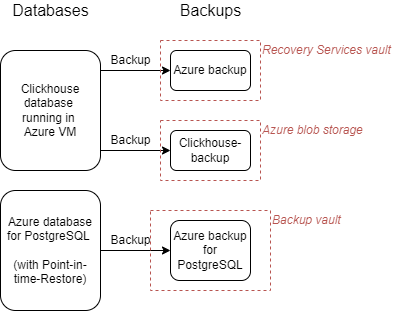
\includegraphics[width=.9\linewidth]{figures/Backupsolution.png}
    \caption{Illustration of the databases and their backup solutions}
    \label{fig:backup_architecture}
\end{figure}

\subsection{Test environments for ClickHouse}
%as well as our rationale for choosing which solutions to test.
\subsubsection{Test environment for non-performance sensitive tests} \label{method:ch-non-perf}
In order to perform experiments where performance was not being measured,
we set up a simple test environment.
The test environment consisted of a single Linux VM running Ubuntu 16.04.
The VM size selected was "Standard B1s" \cite{rishabv90_b-series_nodate}, which is a general purpose VM with
a single vCPU, 1GB of RAM, and a 30GB SSD. 
ClickHouse and clickhouse-backup was installed on the VM and configured. In addition, Azure Backup was set up. A data set of around 700MB (when compressed by ClickHouse) was used. A detailed overview of how the non-performance critical test environment was set up is included in the appendix, see \ref{app:ch-non-perf}.

\subsubsection{Test environment for performance tests}

For performance tests,
a different test environment was used.
A more powerful VM was necessary in order to 
avoid bottlenecks that could interfere with the performance test results.
The VM size selected was "Standard D4s v4" \cite{andysports8_dv4_nodate}.
This is a general purpose VM with 4 vCPUs and 16GB of RAM.
16GB of RAM is less than the amount recommended for ClickHouse \cite{noauthor_usage_nodate} but greater than the minimum requirement \cite{noauthor_requirements_nodate}.
The reason we chose this VM size was because it was the largest size available with our Azure subscriptions vCPU quota.
This is unfortunate, but we believe it was sufficient for our tests.

The OS disk size selected was 2048GB, which was enough to leave some overhead after loading the test data. The uncompressed size on disk of the data set used was around 5TB. The data set was compressed to a size of 955GB by ClickHouse. We believe this amount of data should be enough to give a realistic overview of the performance of each backup solution.

For a detailed overview of how the performance test environment was set up, 
see \ref{app:ch-perf} in the appendix.

\subsection{Test environment for PostgreSQL}
We tested Azure database for PostgreSQL with the \texttt{GP\_Gen5\_2}-SKU, a general purpose configuration that is similar to the needs of most businesses. The setup was done with a PowerShell script for repeatability, and can be seen in appendix \ref{pg_setup}. Point-in-time-restore is enabled by default (and can not be disabled.) 

Connecting to the PostgreSQL instance was done with pgAdmin 4.
This is a tool used to manage PostgreSQL databases.
Another option here would have been using Azure Data Studio.
% which would require installing the PostgreSQL extension. 

We populated the database with data using a script.
See appendix \ref{pg_populate} for details.
%in order to show data loss and restoration in the experiments. 

In order to protect PostgreSQL with Azure Backup, we created a Backup vault and deployed a backup instance with an accompanying backup policy for the PostgreSQL server within it. 
The process is described in detail in appendix \ref{pg_azurebackup}. 

\section{Scenarios} \label{Scenarios}
In order to evaluate the effectiveness of each of the backup solutions, we came up with three practical scenarios. These are imagined attacks against the databases or backups, which the backup architecture has to be able to withstand.

These scenarios were used as a basis to create experiments, which are practical demonstrations of how an attack could be carried out, and how the system would recover from the attack, or otherwise how the risk of the attack may be mitigated. The scenarios are also used to provide a meaningful context for discussing each backup solution's resistance to ransomware. 

\subsection{Scenario 1: Attacker encrypts database data}

This first scenario is perhaps the most central scenario for the project.
This is essentially a basic ransomware attack, where only the data stored on the database servers are encrypted.
This attack is illustrated in figure \ref{fig:scenario 1}.

\begin{figure}[h!]
    \centering
    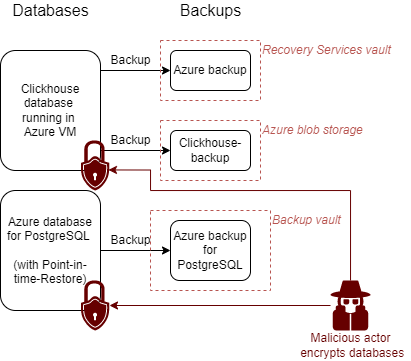
\includegraphics[width=.9\linewidth]{figures/Scenario1.png}
    \caption{Illustration of Scenario 1, a malicious attacker encrypting databases}
    \label{fig:scenario 1}
\end{figure}


\subsubsection{Conditions}
This scenario assumed an attacker has managed to gain access to the database-server, or the server that configures it. The attacker has also managed to elevate their privileges enough to delete or encrypt data. The attacker is not necessarily sophisticated enough to look further into the system,
or attempt to counteract the security controls in place. 

\subsubsection{Consequences}
The worst case consequences of this scenario is complete data loss.
Given that the attackers are using a modern strain of 
ransomware with sophisticated encryption schemes,
as it is fair to assume, the encrypted data could be completely lost.
This attack without a plan for data restoration could force the 
victim organisation to pay the ransom or risk bankruptcy 
especially if the data is business-critical. 

\subsubsection{Risk Mitigation}
Recovering from this attack involves restoring the data in the databases from backup. As the goal of the attack is to ensure the organisation loses access to their data, and making the ransom the only viable method of recovery, our goal should be to ensure another method of recovery exists. 

In our case, recovery from this scenario involved verifying that the backup solutions reliably backed up data, and that the data restored from them was the same as we backed up. 

\subsubsection{Testing}
To test this scenario we encrypted or deleted data in each database. Each of these has backups that we then restored from. In addition to testing that restoring from these backups works, we noted significant aspects of the recovery process in order to better evaluate the non-functional attributes of the backups. 

\paragraph{ClickHouse experiment:} 

To test this scenario with ClickHouse, we ran an experiment where we encrypted certain files in \texttt{/var/lib/clickhouse/}. This is the default storage path for ClickHouse. The files were encrypted using an encryption tool called \texttt{ccrypt}. The full details of how this experiment was conducted can be found in section \ref{app:chs1e1} of the appendix.

A short summary follows here.\\

\noindent
The files we encrypted were files that correspond to columns in a database table.
We tried encrypting both a single file and the whole directory containing the files.
The effects the encryption had on the database were observed.
Then, the database was recovered using backups from clickhouse-backup and Azure Backup.

The following files were encrypted:

\begin{itemize}
    \item \path{/var/lib/clickhouse/store/c28/c283470d-9ab3-4be8-bd81-132274c9f9b0/all_1_35_2/radio.bin}
    \item \path{/var/lib/clickhouse/store/}
\end{itemize}

\paragraph{PostgreSQL experiments:} % [TODO] Åsmund eller Omer les gjennom og godkjenn endringer
We find it unlikely that a normal ransomware virus would be able 
to encrypt data in a managed PostgreSQL database. It is however not unlikely that future threat actors target managed cloud services to a greater degree than is normal now, as more organisations move to the cloud
To test this scenario we will, instead of encrypting tables, 
simulate an attack where the tables in the database are dropped.
This gives us an opportunity to test how recovery is performed with each backup solution.


The first backup method that was tested was Point-in-time restore (PITR).
The table was dropped and then restored with PITR.
The experiment is described in detail in the appendix (\ref{app_pg_s1e1}). 
%In this experiment we used the built-in PITR feature,
%and restored to a new database server instance in order to restore the data in a safe environment. 

To test recovery with Azure Backup for PostgreSQL,
we once again dropped the table and started recovery.
The Backup vault GUI for Azure Backup for PostgreSQL was used to restore to a new database from the latest backup available.
This is described in detail in appendix \ref{app_pg_s1e2}.

\subsection{Scenario 2: Attacker deletes backups}
In a human-operated ransomware attack, it is likely that the attacker would attempt
to delete backups before deploying the ransomware itself. Figure \ref{fig:scenario 2} shows the attacker deleting the backups in our test environment. 
\begin{figure}[h!]
    \centering
    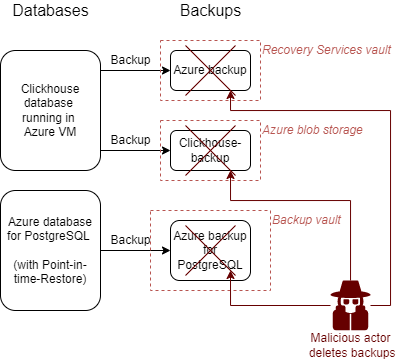
\includegraphics[width=.9\linewidth]{figures/Scenario2.png}
    \caption{Illustration of Scenario 2, a malicious attacker deleting backups}
    \label{fig:scenario 2}
\end{figure}

\subsubsection{Conditions}
The attacker would need access rights at a high enough level to threaten the backups. Whereas in scenario 1 the attacker only needed access to the specific data they attempted to ransom, the attacker would in this scenario also require access to the backup administrator's Azure account, or an account with equivalent privileges over the backups.   

\subsubsection{Consequences}
This attack is unlikely to be devastating on its own, 
but if the attacker is able to delete or encrypt the data in the databases as well, 
this could be crippling for an organisation. 
The ultimate consequence of such an attack would be total data loss.

\subsubsection{Risk Mitigation}
Preventing this scenario from even occurring is critical to any backup implementation. If for example a compromised administrator has access to both the database and the backup, they become a single point of failure for the whole system. 

A number of attacks may be avoided if there are routines to monitor logs and alerts that may tell the organisation that something is wrong. Even if an attacker is able to bypass the security features protecting the backups, there ought to still be someone monitoring any log entries or alerts that this is happening. This would let the organisation preemptively try to mitigate the attack, and ideally lock the attackers out of the network.

Even if the backups are deleted, they may still be recoverable. By default Recovery service vaults has soft delete (see \ref{Soft Delete}) enabled, which would allow the organisation to recover their backups, and then recover their data from them. Note that Backup vaults do not supports soft delete. Soft delete can also be enabled for Azure Storage Blobs.

\subsubsection{Testing} 
In order to test this scenario, we attempted to delete backups made with the different backup solutions.
After this we attempted to restore them and recover data from the now undeleted backups.
Where that was not possible we also looked into other security mitigation possibilities.

\paragraph{ClickHouse experiments:} 

For ClickHouse, four experiments were performed.
These all involved destroying backups in different ways.

In the first experiment, local backups made with clickhouse-backup were encrypted using the tool \texttt{ccrypt}, and the results were observed. We attempted to list and restore the encrypted backup using \texttt{clickhouse backup list} and \texttt{clickhouse backup restore} respectively. See the appendix (\ref{app:chs2e1}) for full details regarding how the experiment was carried out.

Clickhouse-backup has commands for deleting local and remote backups 
(\texttt{clickhouse-backup delete [local/remote]}).
In the second experiment, backups made using clickhouse-backup were deleted using these commands.
This was done in order to simulate an attack where the attacker has root access to the VM,
but not to the Azure environment itself.
Afterwards, the deleted backups were recovered by
undeleting the Blobs via the Azure CLI,
and then restoring the database with \texttt{clickhouse-backup restore\_remote}.
See the appendix (\ref{app:chs2e2}) for the full details.

The third experiment was similar to the second, 
in that remote backups made using clickhouse-backup were deleted.
This time, they were deleted  using the Azure CLI,
in order to simulate an attack where  the attack has access to an Azure Cloud Shell session.
Afterwards, the backups were once again recovered by undeleting
the Blobs using the Azure CLI and then restoring the database with \texttt{clickhouse-backup restore\_remote}.
See the appendix (\ref{app:chs2e3}) for the full details.

In the fourth experiment, backups made using Azure Backup were
deleted, and then restored from their soft deleted state.
Both deletion and restoration was performed using the Azure CLI.
See the appendix (\ref{app:chs2e4}) for the full details.


\paragraph{PostgreSQL experiments}
Backups for a managed PostgreSQL database are inherently tied to the database, due to its point-in-time restore (PITR) function. To test this scenario, we therefore deleted the database server instance in an attempt to delete the backup, and then restored it from PITR. When creating a new managed PostgreSQL Azure Database the option is given to restore from a PITR-point. This allows the database to be "undeleted" in practice, as long as it is restored within the restore period. This process is shown in \ref{app_pg_s2e1}.

As Backup vaults, which Azure Backup for PostgreSQL uses, does not support soft delete functionality, the experiment for the Azure Backup solution was simply to delete the backup instance in the Backup vault. %The process is described in detail in appendix \ref{app_pg_s2e3}.
After doing so, there was no option to undelete or restore the backup data. 

In addition to restoring the deleted backups, one important risk mitigation effort would be to ensure that the backup administrator is alerted when backup data is deleted. 
Azure Database for PostgreSQL does not automatically alert the backup administrator when backup data is deleted.
Alerts will also have to be monitored elsewhere than the Backup Center, as no alerts have shown up here throughout our testing.

We created an Alert Rule that sent an alert each time the "Microsoft.DataPro-tection/backupVaults/backupInstances/delete" action succeeded within the scope of the subscription containing the Backup vault. This is the action which deletes backup instances in backup vaults. This rule was linked to an Action Group that sent an email to the backup administrator each time the Alert was delivered. This could also be sent as a phone notification or a text message. This alert rule is described in detail in appendix \ref{app_pg_s2e2}. 

\subsection{Scenario 3: Backup administrator compromised}
The third scenario assumes a complete compromise of the backup administrator account.
This account has administrator access to the vaults in Azure,
or has other permissions allowing them to modify or delete backups, or change security settings.
In the previous scenario we looked at how to mitigate risks associated with a lost or deleted backup. This time the attacker has access to the backup administrator account and can disable whatever security settings or delete whichever resources they wish. 

This attack is illustrated in figure \ref{fig:scenario 3}, which shows the backup administrator account controlled by the malicious actor, as well as the domain which the backup admin account controls.

\begin{figure}[h!]
    \centering
    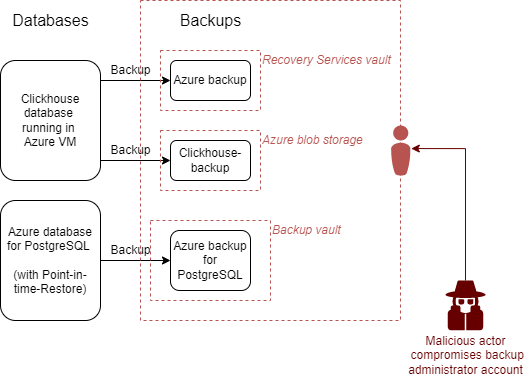
\includegraphics[width=.9\linewidth]{figures/Scenario3.png}
    \caption{Illustration of Scenario 3, a malicious attacker compromising backup admin}
    \label{fig:scenario 3}
\end{figure}

\subsubsection{Conditions}

The condition for this scenario to occur is simply that an attacker has gained access to the backup administrator account. As discussed in section \ref{ZeroTrust}, this can easily happen through simple human error, or misuse of administrator accounts when performing mundane tasks.

\subsubsection{Consequences}
One of the consequences of this scenario is the permanent loss of all data, given that the attacker is able to disable soft delete and delete all backups and deploy ransomware shortly thereafter. Ransomware operators spend weeks trying to figure out all there is to know about an organization, and if they see an opportunity to attack both the databases and their backups simultaneously, they are sure to grab it. 

\subsubsection{Risk mitigation}
There are security features in Azure to prevent a compromised administrator account from disabling soft-delete and deleting backups. One of them is Multi-user authorization, as described in \ref{MUAtheory}. In addition to that feature in particular, well designed access control in general, based on Role-based access control, and Zero-trust features such as Just-in-time access can prevent this scenario from resulting in any major consequences.
 
\subsubsection{Testing}
Testing for this scenario involved exploring how much data could be made irrecoverable with full access to the backup resources in Azure, 

\paragraph{ClickHouse experiments:}

We performed 3 experiments for this scenario in Clickhouse.

In the first experiment, 
soft delete was disabled for a protected item in Azure Backup before the item was deleted using the Azure CLI.
See the appendix (\ref{app:chs3e1}) for the full details.

In the second experiment, the entire Recovery Services vault used to store Azure Backup backups
was deleted using a PowerShell script.
See the appendix (\ref{app:chs3e2}) for the full details.

In the third experiment, we once again attempted to run the Recovery Services vault deletion script,
but before doing so, we enabled Multi-user authorization and observed what happened.
See the appendix (\ref{app:chs3e3}) for the full details.

\paragraph{PostgreSQL experiments:} \label{pg_sc3}
Since there it is not possible to disable the soft delete feature of PITR, this scenario is less relevant for PostgreSQL compared to ClickHouse. Backup vaults support neither soft delete nor MUA, so this scenario does not have a direct solution using Azure Backup either.  

\section{Performance testing} \label{Perftest}

In order to determine whether it is realistic that a backup solution 
is able to recover data within a given RTO,
we conducted performance tests for each backup solution.
The performance tests measure how long it takes to restore a database of a certain size.
This is a useful parameter to consider when comparing the different backup solutions.  

\subsection{Performance tests for ClickHouse}
ClickHouse is able to handle large amounts of data,
which means a backup solution for ClickHouse should also be able to.
We decided to load ClickHouse with 1TB (compressed) of data,
which we believe was enough to get a realistic idea of
the backup solutions' performance.

For the Azure Backup test, we first prepared the environment by deleting the VM, listing the available restore points, and then selecting which restore point to use. A stopwatch was started the moment we initiated the restore job. The stopwatch was stopped when it was possible to connect to the VM using SSH and run database queries. The time used by the restore job itself is printed of the command 
\noindent \texttt{Restore-AzRecoveryServicesBackupItem}.
This was noted separately.
See \ref{app:chab-perf} in the appendix for the full details regarding how the tests were performed.

For clickhouse-backup, the plan was to measure the time it took to create a new VM with the necessary software,
using a stopwatch.
Then, the builtin command \texttt{time} was to be used to measure the time used by the
\texttt{clickhouse-backup restore\_remote}.
Afterwards, the times were to be summed up to get the total restore time.
However, we experienced errors we were not able to resolve, which prevented us from carrying out the test.
Appendix \ref{app:chbk-perf} contains details about how the tests were performed,
and what went wrong.
This is also discussed in chapter \ref{Results}.

%, we first measured the time it took to create a new VM and install the necessary software with a stopwatch. Then we used the builtin shell command \texttt{time} was used to measure the time used by the command  \texttt{clickhouse-backup restore\_remote}. The times were then summed up. See \ref{app:chbk-perf} in the appendix for the full details regarding how the tests were performed.

\subsection{Performance tests for PostgreSQL}

The following experiments compared the performance of Azure Database for PostgreSQL single server when restoring using different methods. A general purpose single server with 4 vCores and 100 GB of storage was deployed in the same way as for our other testing, as seen in \ref{pg_setup}.

We populated the databases with data using a script (see appendix \ref{pg_populate}). 
The script generated 7107MB of data.

% Connecting to the database using pgadmin4 and running the psql command below returned a size of 7107 MB.
% 
% \begin{minted}[breaklines=true,breakanywhere=true]{sql}
% SELECT pg_size_pretty( pg_database_size('postgres') );
% \end{minted} 


\subsubsection{Delete server and restore using backup vault}

After deleting the data in the database we recorded how long it took to restore the data to a running PostgreSQL-instance. 

%If archive then could take longer,.. Backup vault test was performed a newly full backup, while PITR uses transactional history as well as differential backups to build back to a previous state.

HER TRENGS DET Å SKRIVES MER/TYDELIGERE.

This was sufficient for a baseline test. Further, a key vault was deployed which the backup vault linked to for access to the connection string necessary to work with the PostgreSQL single server. 

The goal was measuring the restore time after deleting a server. 

\subsubsection{Delete server and restore using point-in-time restore}

A test similar to the previous was performed with point-in-time Restore.
PITR has an option to create a new server from the restore point,
which is what was used in this test.

% Azure has the option of point-in-time restore to a new server which is tested out with the same database and single server configuration as the one used in the backup vault performance test above. The difference in implementation was that PITR creates a new server as part of the restore process, while the same has to be done as a separate operation for backup vault.
